% Co jsem udělal já
\chapter{Návrh zařízení ($\Sigma$ = 22 stran)}
\section{Princip funkce navrženého systému ($\sum$ = 3 strany)}\label{sec:PopisFunkceSystemu}
% \purpose{Tady bych rád popsal, jak to bude celé fungovat.}

Celý systém je primárně navržen kolem mobilní aplikace, jelikož požadavek na dálkové řízení dopravníků je jeden ze základních požadavků navrženého systému.

Aplikace bude obsahovat stránku pro plynulou WiFi komunikaci s vývojovou deskou WEMOS D1 Mini Pro. Vývojová deska je připevněna k desce plošných spojů, která je třemi kabely připojena na ovládací panel (2 datové kabely a 1 napájecí). Tímto způsobem může deska nastavovat takové digitální vstupy, k ovládání dopravníku.

Ovládací panel frekvenčního měniče si následně dle jeho nastavení podle své konfigurace interpretuje tyto příkazy a řídí výkonovou část frekvenčního měniče pro ovládání asynchronních motorů.

Na obrázku \ref{fig:PrincipFunkceZarizeni} je schéma základního principu.

\begin{figure}[hptb]
	\centering
	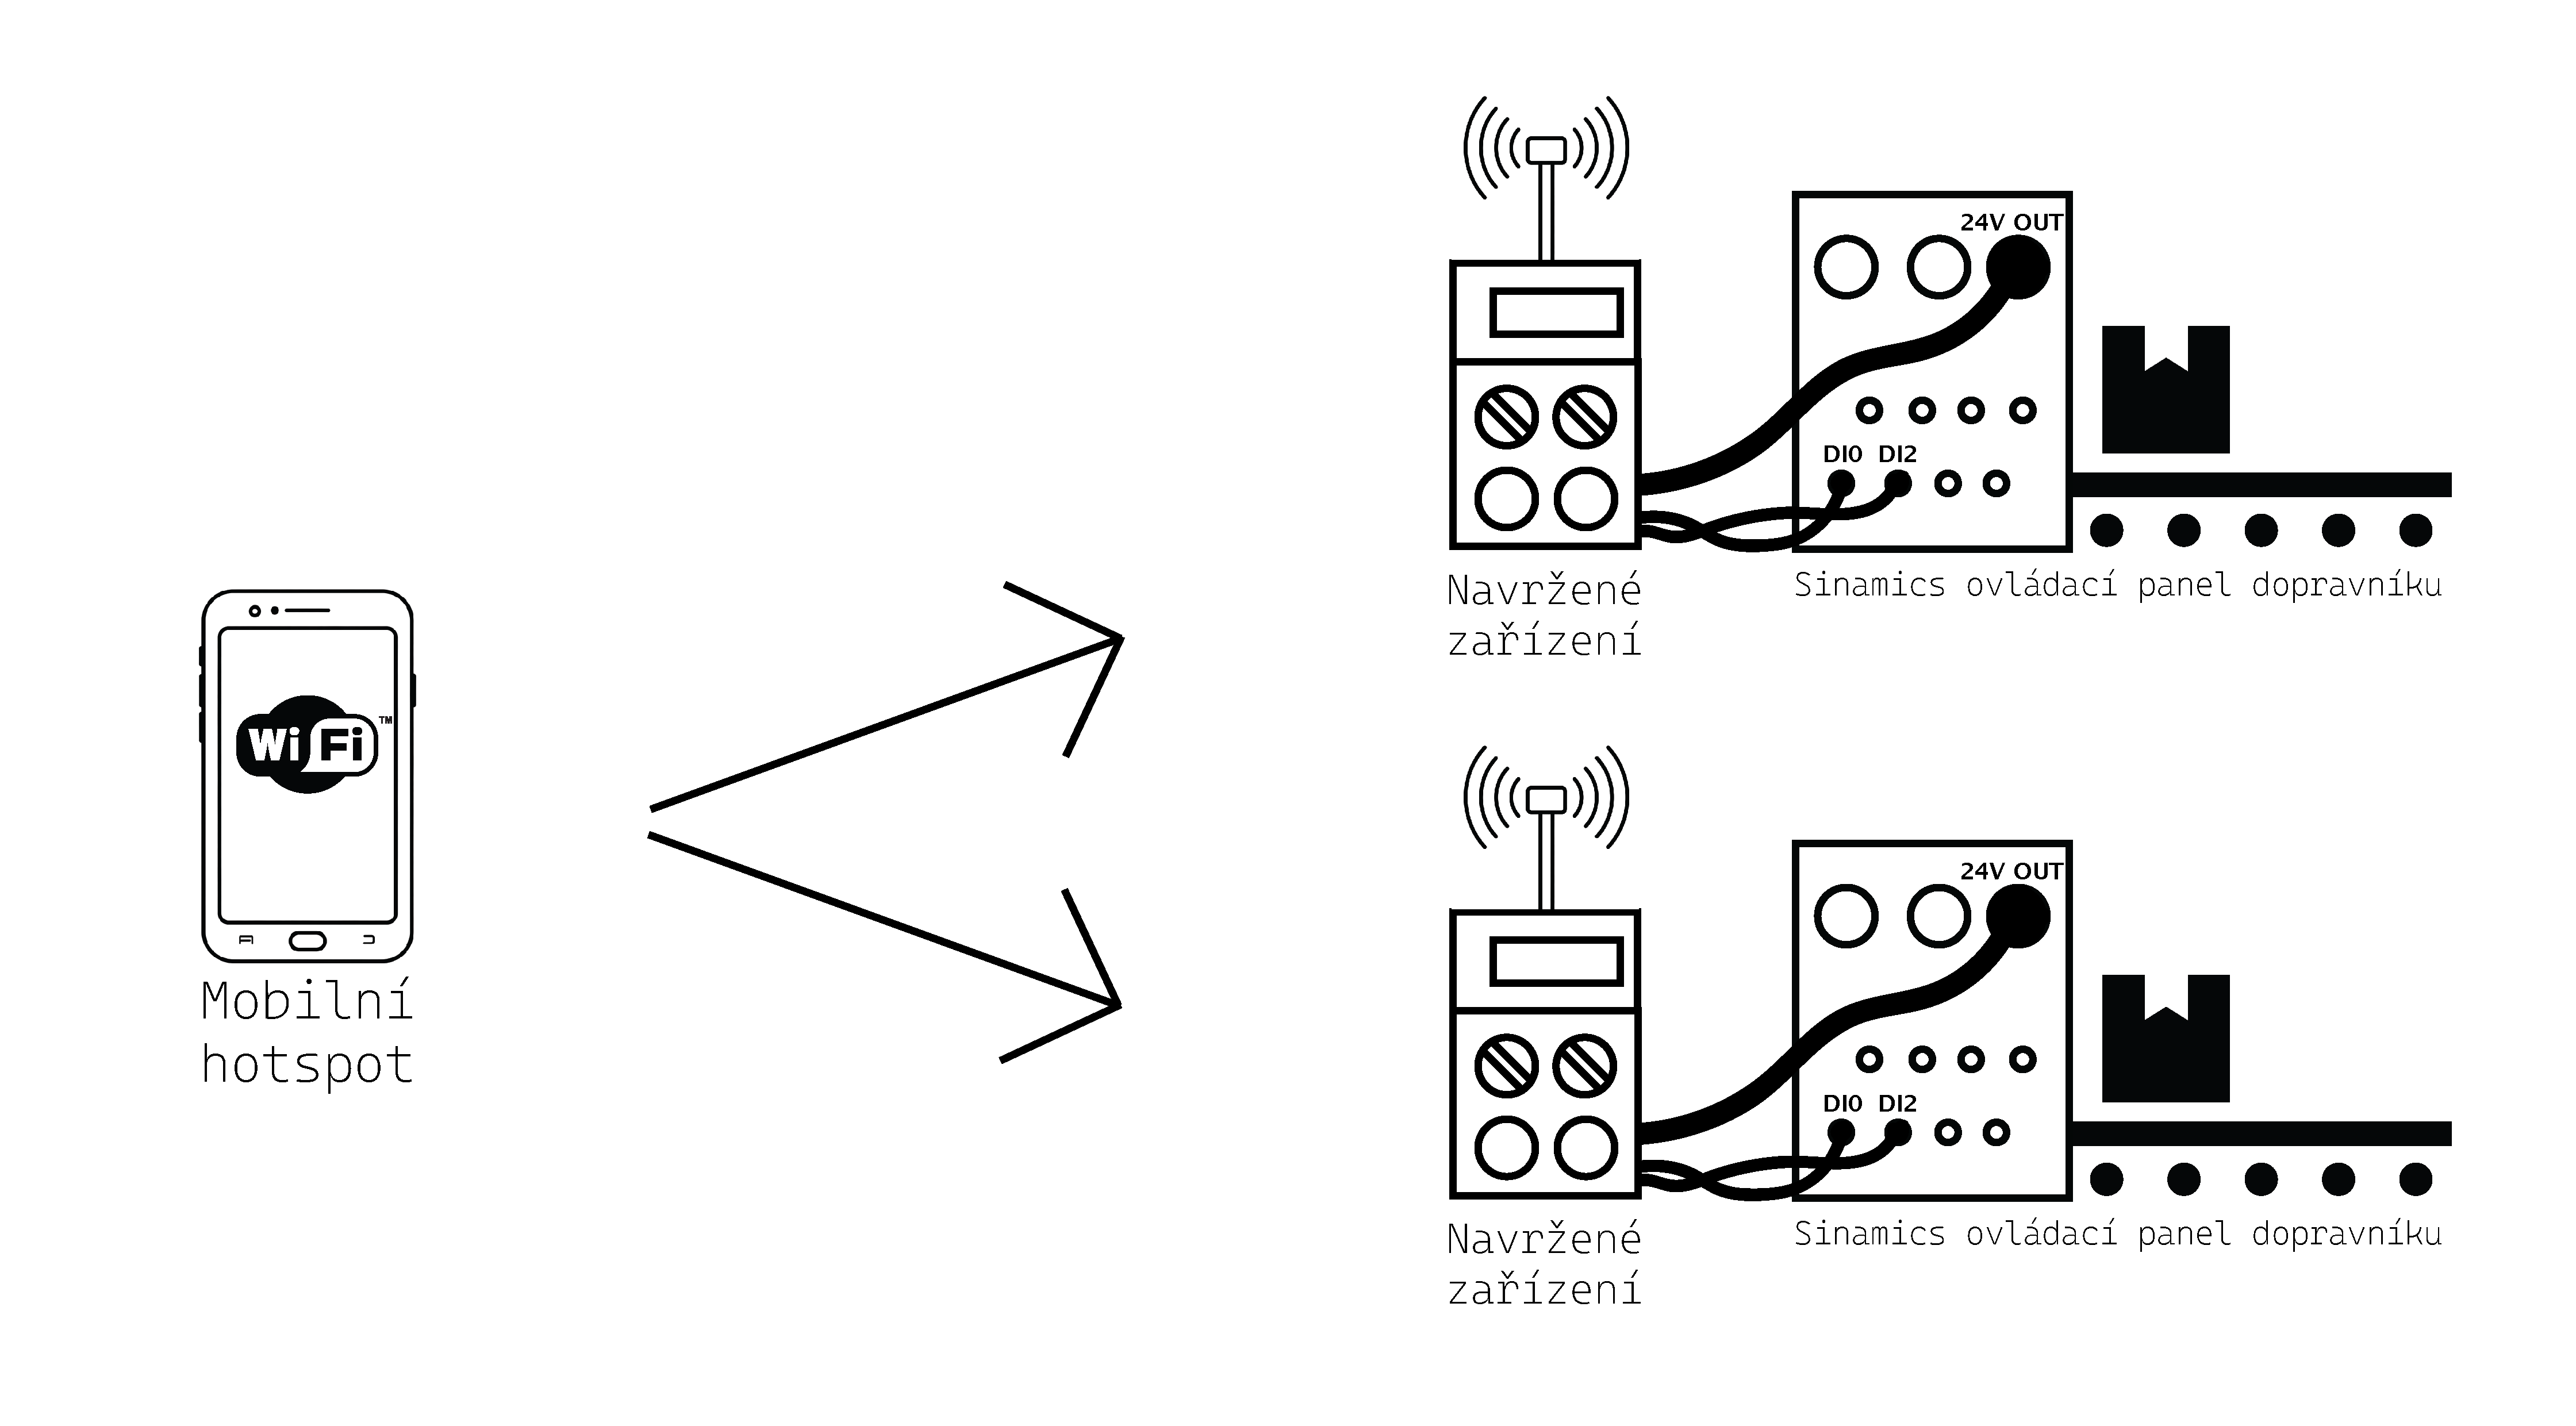
\includegraphics[width=1\linewidth]{images/FunkcniSchema_DvaOvladace.png}
	\caption{Schéma principu jak navržený systém funguje}
	\label{fig:PrincipFunkceZarizeni}
\end{figure}

Jelikož mobilní aplikace komunikuje s vývojovými deskami pomocí WiFi, je potřebné aby se buďto mobilní zařízení připojilo na přístupové místo vývojové desky, anebo se může vývojová deska připojit na hotspot mobilního zařízení. WebServer umožňuje obě varianty. Pro účely tohoto systému se více hodí ta druhá možnost, protože přirozeně umožňuje mít jeden hotspot na mobilním zařízení a na ten se může připojit více vývojových desek. Tohle umožňuje jednoduše ovládat více dopravníků zároveň. Další výhoda je, že vývojové desky připojené na hotspot vůbec nevyužívají toho, že je mobilní telefon připojený k internetu a tak nijak nezatěžují rychlost připojení - jediná limitace počtu takto připojených vývojových desek je tedy limitace maximálního počtu co může mít mobilní telefon připojené přes hotspot. Nevýhoda tohoto způsobu komunikace je ovšem taková, že se musí nastavit jednotné jméno a heslo WiFi komunikace, které bude zadané přímo ve firmwaru vývojové desky a pokud bude potřebné tyhle údaje změnit, bude se muset přehrát kód všech vývojových desek (pro všech pět používaných zařízení).

Díky tomu, že je tento systém navržený tak, aby přes 5-pinové kabely spínal digitální vstupy ovládacího panelu, je tento systém možné použít i na frekvenční měniče jiných značek než je Sinamics. Kabely, které se používají pro komunikaci s ovládacím panelem frekvenčního měniče (M12 5-pinové kabely) jsou v dnešní době u frekvenčních měničů časté. Jediné co je tedy potřeba pro používání systému s jiným frekvenčním měničem jsou správné konektory a dále aby bylo možné vyresetovat ovládací panel do podobného výchozího nastavení jako má Sinamics CU240-2.

Na obrázku \ref{fig:PopisZarizeniCoOvladaDopravnik}  je finální vzhled schránky na desku plošných spojů s tlačítky, LCD displejem a dalšími funkcemi. Deska je dále popsaná v kapitole \ref{sec:Hardware}.

\begin{figure}[hptb]
	\centering
	\includegraphics[width=0.5\linewidth]{images/obrazekKrabicky_annot.png}
	\caption{Popis zařízení co ovládá dopravník}
	\label{fig:PopisZarizeniCoOvladaDopravnik}
\end{figure}

Na obrázku \ref{fig:MobilniAppScreenshots} je finální vzhled mobilní aplikace. Jsou zde vidět tři hlavní strany aplikace - Nastavení, Pomoc a Ovládání. Ovládání komunikuje s vývojovou deskou tím že posílá příkazy pro ovládání dopravníku, ale také získává průběrná data o rychlosti dopravníku a typu ovládání (lokální nebo dálkové). Aplikace je dále popsaná v kapitole \ref{sec:SoftwareVMobilniAplikaci}.

\begin{figure}[hptb]
	\centering
	\begin{subfigure}[t]{0.3\textwidth}
		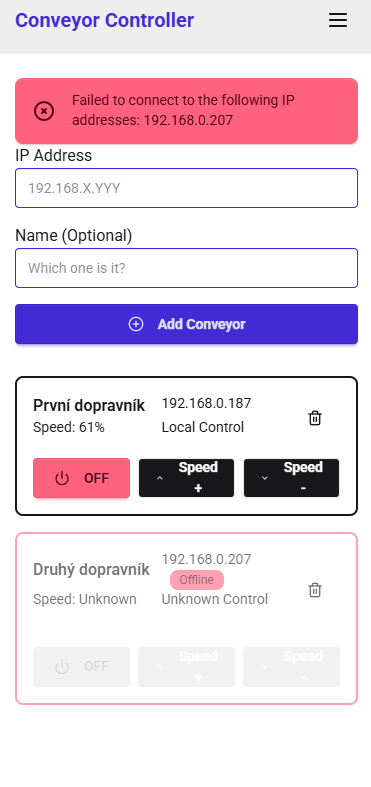
\includegraphics[width=\textwidth, height=290px]{images/MobilniLanding.png}
		\caption{Vstupní stránka aplikace}
		\label{fig:MobilniLanding}
	\end{subfigure}%
	\begin{subfigure}[t]{0.3\textwidth}
		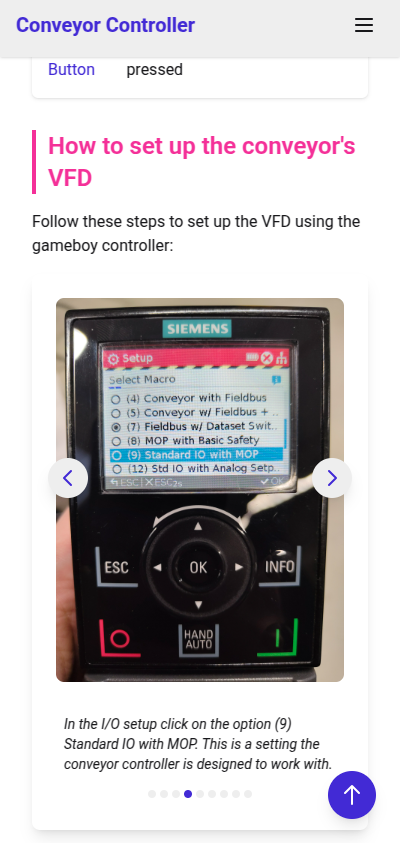
\includegraphics[width=\textwidth, height=290px]{images/MobilniSetup.png}
		\caption{Část stránky nastavení}
		\label{fig:MobilniSetup}
	\end{subfigure}%
	\begin{subfigure}[t]{0.3\textwidth}
		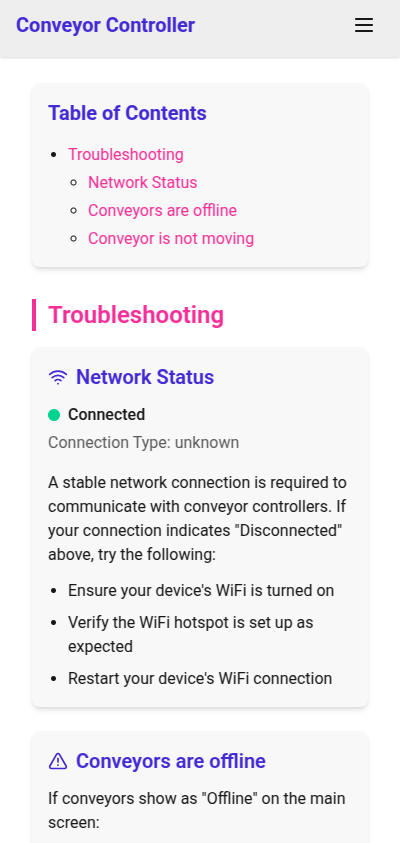
\includegraphics[width=\textwidth, height=290px]{images/MobilniHelp.png}
		\caption{Část stránky s častými chybami}
		\label{fig:MobilniHelp}
	\end{subfigure}
	\caption{Vysílat příkazy zařízení bude mobilní aplikace připojená přes hotspot}
	\label{fig:MobilniAppScreenshots}
\end{figure}

\subsection{Požadavky na systém (0.5 strany)}\label{sec:PozadavkyNaSystem}
Pro zajištění funkčnosti a smysluplnosti návrhu je nutné si stanovit některé požadavky, které by systém měl splňovat. Tyto požadavky reflektují nejenom požadavky od společnosti Honeywell, ale i požadavky na základní spolehlivost, jednoduchost a bezpečnost ovládání dopravníků tímto způsobem.

Zde jsou požadavky, které by implementace navrženého zařízení měla splňovat:

\begin{itemize}
    \item \textbf{Lokální a dálkové ovládání}\\
    Systém bude schopný ovládat dopravníky nejenom lokálně ale i bezdrátově.
    \item \textbf{Ovládání více dopravníků zároveň}\\
    Systém by měl jednoduše zprostředkovat ovládání více dopravníků zároveň.
    \item \textbf{Ovládání z mobilního zařízení}\\
    Aby se minimalizoval počet potřebných zařízení se systém musí dát provozovat z mobilního zařízení pomocí WiFi hotspotu.
    \item \textbf{Napájení z ovládacího panelu}\\
    Systém musí být navržený tak aby jeho rozšířené funkce bylo možné napájet připojením na $24V$ výstupní port v ovládacím panelu.
    \item \textbf{Systém musí mít ovládání které je čistě analogové}\\
    Systém by měl být navržen tak, aby bylo stále možné dopravníky ovládat i pokud by něco zamezovalo napájení vývojové desky.
    \item \textbf{Uživatelská přívětivost systému}\\
    Systém by měl být uživatelsky přívětivý a jeho nastavení by mělo být jednoduše dostupné pro uživatele spolu se všemi informacemi jak s ním pracovat.
\end{itemize}

\section{Hardware ($\Sigma$ = 3 strany)}\label{sec:Hardware}
% \purpose{Jak jsem postupoval při návrhu a jak ta finální verze vypadá}

Základní stavební kámen celého systému je jeho hardware společně s deskou plošných spojů (DPS) ve které je umístěn. Celé zapojení bylo nejdříve navržené jako elektrické schéma. To bylo postupně vylepšováno, později předěláno do schématu v programu pro tvorbu DPS a nakonec bylo vytvořené rozložení komponentů přímo na desce. Pozdější verze návrhu byly provedeny v počítačovém programu na návrh desek plošných spojů jménem KiCAD. Blokové schéma funkčnosti desky lze vidět na obrázku \ref{fig:SchemaDesky}.

\begin{figure}[hptb]
	\centering
	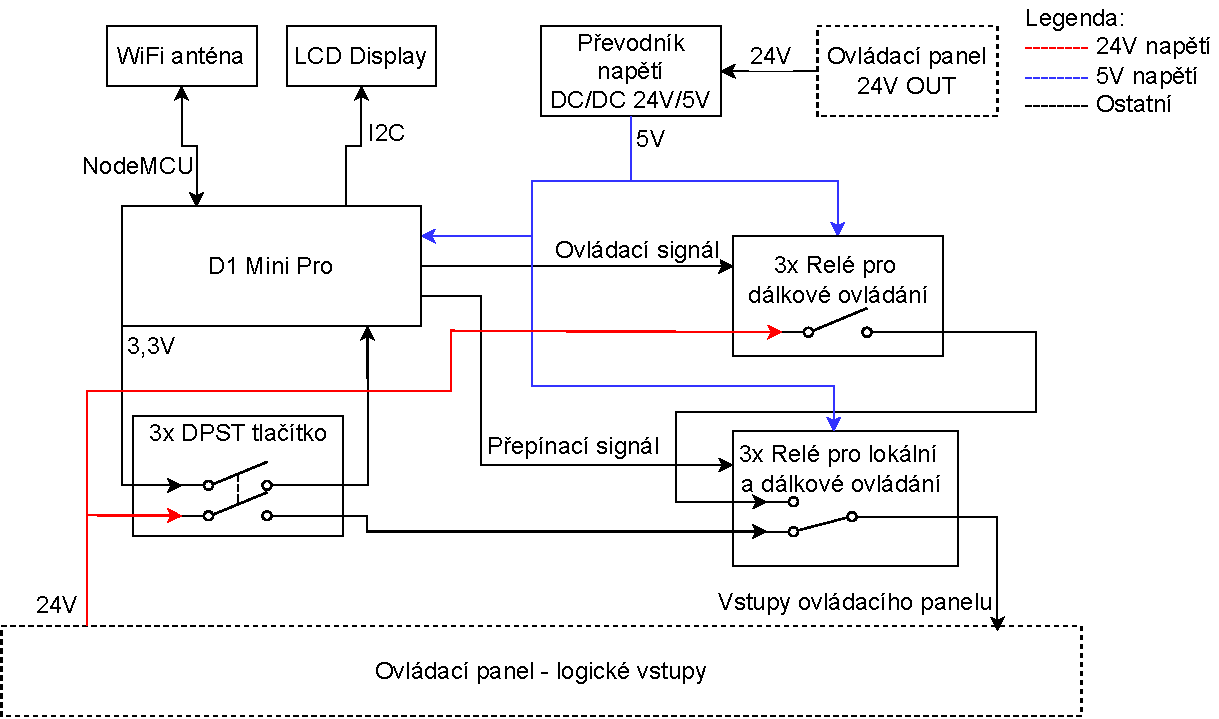
\includegraphics[width=1\linewidth]{images/Electrical_Schematic_V2.drawio.pdf}
	\caption{Blokové schéma desky plošných spojů}
	\label{fig:SchemaDesky}
\end{figure}

Při tvorbě desky se vycházelo z požadavků na systém. Nejdřív se vycházelo z toho, že desku musí být možné napájet z ovládacího panelu, který má výstupní port na kterém je $24V$ a který je schopný dodat maximálně $8A$. Ze začátku se tedy počítalo s $24V$ napětím, pro které bylo potřeba zvolit dobrý převodník napětí co je schopný napětí přeměnit na $5V$ kterým se napájí vývojová deska. Nakonec byl zvolený převodník napětí s galvanicky oddělenou zemí aby se minimalizovala šance, že by kvůli nějaké chybě v návrhu desky byl zničený ovládací panel frekvenčního měniče.
\cite{SiemensG120DGettingStarted}

Dále se při návrhu vycházelo z myšlenky že systém musí mít i lokální i dálkové ovládání, s tím, že lokální ovládání musí být dostupné i bez napájení mikrokontroleru. Tohle bylo vyřešeno návrhem dvou přepínačů. \textit{Relé pro lokální a dálkové ovládání} je přepínač, který je normálně v poloze lokálního ovládání (aby byl splněný požadavek čistě analogového ovládání), ale pokud se na něj přidá napětí, přepne se do stavu dálkového ovládání. Následně je v desce \textit{Relé pro dálkové ovládání}, což je běžné SPST relé které sepne kontakty pokud je na něj přivedeno napětí.

Po dokončení schématu se přešlo na návrh umístění součástek na DPS. Finální návrh lze vidět v obrázku \ref{fig:PCBbothSides}. Při rozmisťování součástek po desce byl kladen důraz na několik kritérií:
\begin{itemize}
	\item Aby měla deska co nejmenší rozměry a měla jen dvě vrstvy
	\item Aby byly všechny součástky na jedné straně desky (jednodušší pájení komponentů na desku)
	\item Aby byly trasy co nejkratší
	\item Aby měla deska co nejméně vertikálních cest (pro zmenšení efektů parazitní kapacity a parazitní indukčnosti)
	\item Aby byly filtrační kondenzátory co nejblíž filtrovaných napájecích vstupů
\end{itemize}

\begin{figure}[hptb]
	\centering
	\begin{subfigure}[t]{0.48\textwidth}
		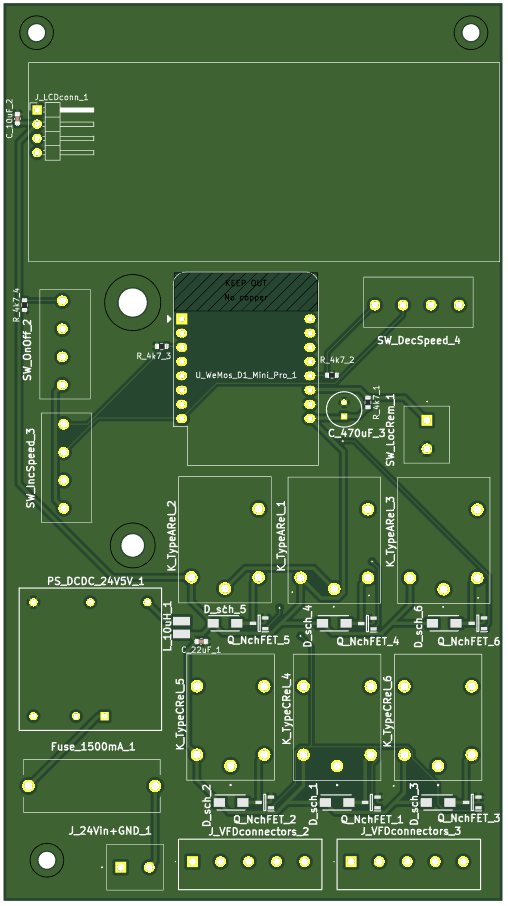
\includegraphics[width=\textwidth]{images/PCBfront.png}
		\caption{Přední strana DPS}
		\label{fig:PCBfront}
	\end{subfigure}%
	\hfill
	\begin{subfigure}[t]{0.48\textwidth}
		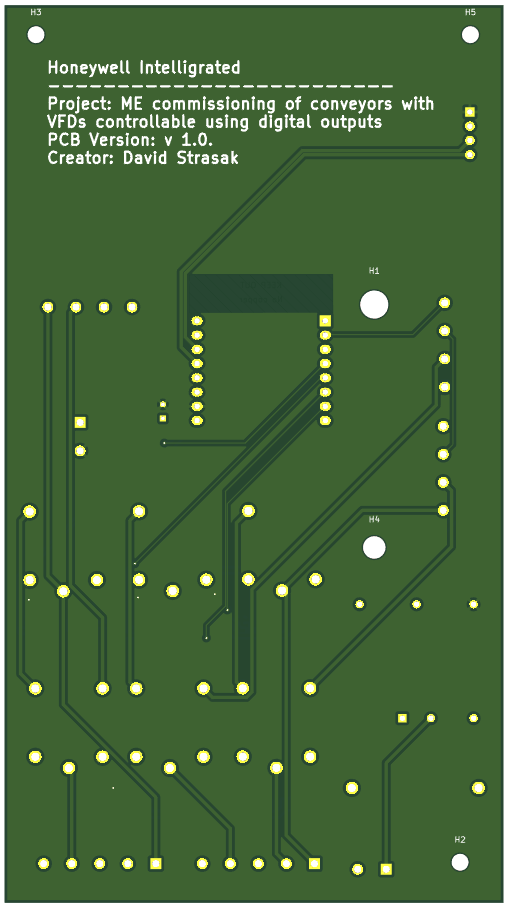
\includegraphics[width=\textwidth]{images/PCBback.png}
		\caption{Zadní strana DPS}
		\label{fig:PCBback}
	\end{subfigure}
	\caption{Návrh desky plošných spojů v KiCAD}
	\label{fig:PCBbothSides}
\end{figure}

\subsection{Ovládání relé}
Jedna z věcí které bylo potřeba vyřešit při návrhu schématu elektrického obvodu je taková, že bylo cílem ovládat relé pomocí výstupních pinů vývojové desky. Pro spuštění relé je ovšem potřeba brát na paměť, že vyžaduje nejenom napětí $5V$ na ovládacím pinu, ale také vyžaduje proud do cívky $133mA$. Vývojová deska je schopná svými výstupními piny poskytnout napětí $5V$, ale její výstupní proud je pouze $10mA$. Tento problém je možné vyřešit pomocí tranzistorů.

Nejjednodušší řešení pro navrženou desku je řešení s N kanálovým NPN tranzistorem MOSFET, jelikož v případě MOSFET tranzistorů obecně stačí aby signál byl napěťový (nemusíme tedy řešit malý proud vycházející z vývojové desky). Nejdřív se relé zapojí tak, aby cívka měla na jedné straně $5V$ napětí a na druhé straně zem. Následně se MOSFET tranzistor dá mezi zem a cívku a na bázi tranzistoru se přivede signál z mikrokontroleru. V tomto zapojení bude skrz relé téct nominální proud, pokud je výstup vývojové desky vysoký, anebo bude obvod rozpojený pokud bude výstup z vývojové desky na nízké hodnotě napětí.

Dále je potřeba ještě paralelně s relé zapojit diodu kvůli ochraně tranzistoru od vybíjecího proudu co cívka generuje po rozpojení obvodu. Tato dioda musí mít v závěrném směru hodnotu napětí vyšší než je $5V$ napětí zdroje a musí se zapojit tak, aby byla otevřená když se otočí polarita napětí na cívce v relé. Pro tuto desku byla zvolena Schottkyho dioda kvůli její rychlosti přepínání a kvůli malému napětí které se na diodě v otevřeném stavu nachází.

Na obrázku \ref{fig:OvladaniRele} je schéma zapojení tohoto způsobu ovládání relé pomocí vývojové desky.

\begin{figure}[hptb]
	\centering
	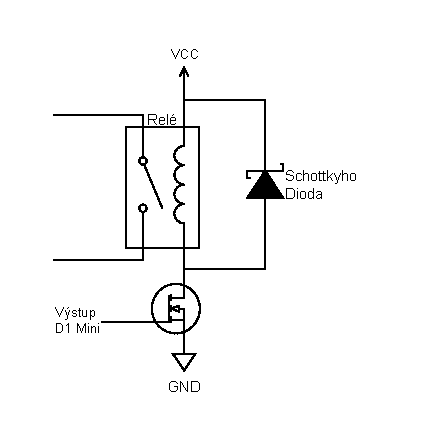
\includegraphics[width=0.6\linewidth]{images/OvladaniRele.drawio.pdf}
	\caption{Elektrické schéma ovládání relé}
	\label{fig:OvladaniRele}
\end{figure}

\subsection{LCD display s I2C převodníkem (1 strana)}
Aby bylo možné celý systém ovládat přes ESP8266 WebServer, je potřebné nějakým způsobem komunikovat s uživatelem IP adresu, kterou má vývojová deska připojená na hotspot mobilního zařízení. Tohle by bylo možné udělat například skrz nastavení multicast DNS na specifickou adresu a tu potom fyzicky napsat na schránku desky. Toto řešení by sice umožnilo přístup k WebServeru, ale neposkytovalo by to další funkce jako systém může mít se zabudovaným LCD displejem do desky plošných spojů.

Použití LCD displeje v systému může uživateli dodávat tyto informace:
\begin{itemize}
	\item Stav připojení mikrokontroleru k hotspotu (před navázáním spojení systém nemůže reagovat na požadavky přes WebServer).
	\item Název (SSID) a heslo hotspotu, které mikrokontroler očekává.
	\item Aktuální rychlost dopravníku.
	\item IP adresu pro přístup k WebServeru.
\end{itemize}

Na základě uvedených důvodů a požadavků na rozsah poskytovaných informací byl pro komunikaci s uživatelem zvolen LCD displej.

Konkrétně byl použit 16x2 znakový LCD displej (obrázek \ref{fig:LcdDisplej}) zakoupený v internetovém obchodě LaskaKit \cite{laskakit_16x2_lcd}. Tento model je vybaven připájeným I2C převodníkem, což zjednodušuje jeho připojení na pouhé čtyři vodiče: dva pro I2C sběrnici (Serial Data (SDA) a Serial Clock (SCL)), jeden pro napájení $5V$ a jeden zemnící vodič (GND). Výhodou zvoleného displeje je také dostupnost knihovny pro Arduino framework, což usnadňuje jeho softwarovou implementaci ve firmwaru mikrokontroleru.
\cite{laskakit_16x2_lcd}

\begin{figure}[hptb]
	\centering
	\begin{subfigure}{0.48\textwidth}
		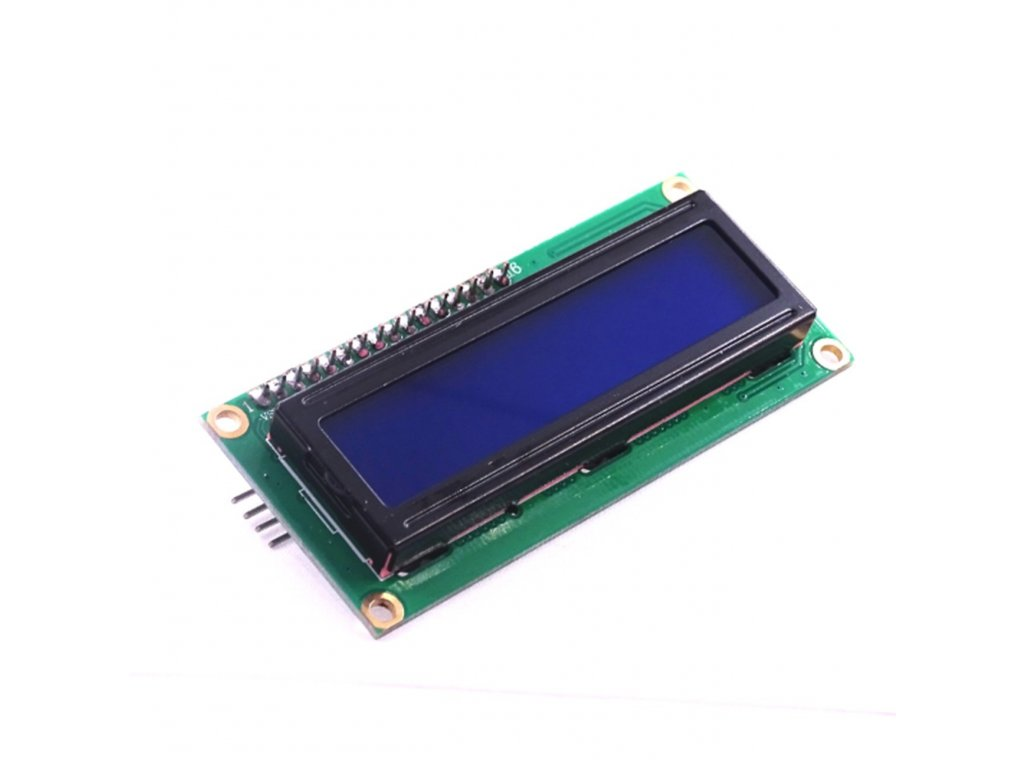
\includegraphics[width=1\textwidth]{images/predni_LCD_s_I2C.jpg}
		\caption{Přední strana}
		\label{fig:PredniLCDDisplej}
	\end{subfigure}
	\hfill
	\begin{subfigure}{0.48\textwidth}
		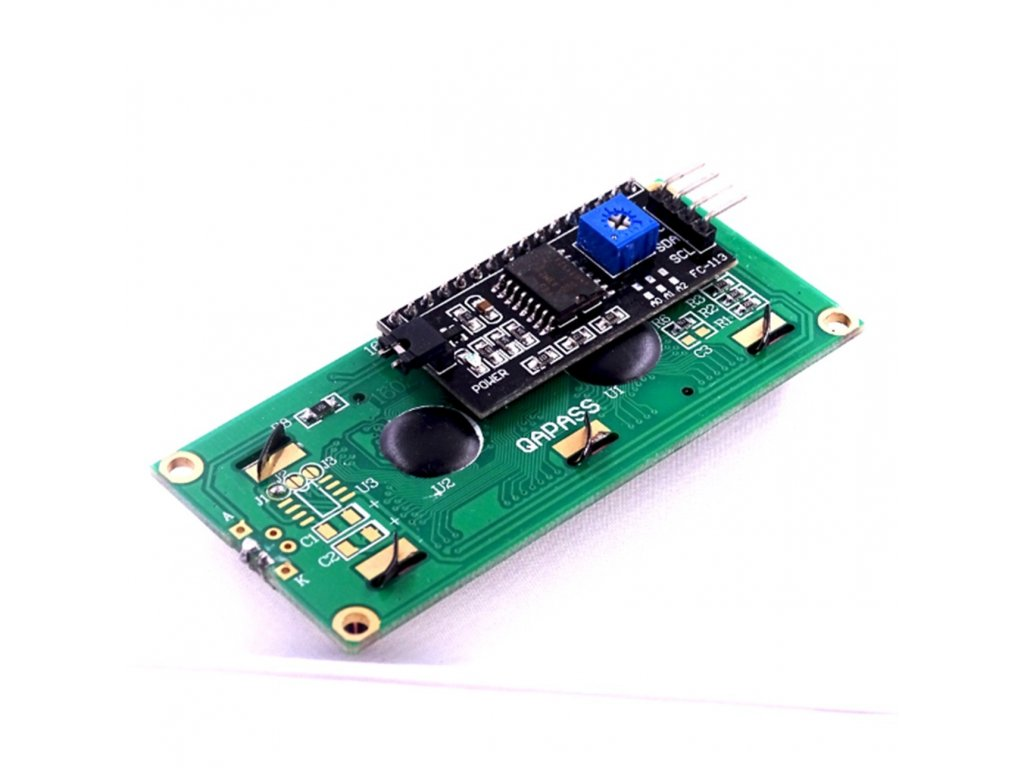
\includegraphics[width=1\textwidth]{images/zadni_LCD_s_I2C.jpg}
		\caption{Zadní strana}
		\label{fig:ZadniLCDDisplej}
	\end{subfigure}
	\caption{LCD displej s I2C převodníkem \cite{laskakit_16x2_lcd}}
	\label{fig:LcdDisplej}
\end{figure}

Vzhledem k citlivosti komunikace po I2C sběrnici na elektromagnetické rušení a přeslechy byly při návrhu desky plošných spojů dodrženy zásady pro minimalizaci smyčkové plochy mezi signálovými cestami SDA a SCL. Tento postup snižuje indukované napětí a přispívá ke spolehlivosti přenosu dat na sběrnici.
\cite{CurrentLoopsBlog}

Pro jednoduchost výměny LCD displeje bylo také zvoleno, že nebude přímo připájený v desce, ale podobně jako vývojová deska bude připojený skrz kolíkové lišty. Tohle zjednodušuje výměnu nebo upravení parametrů LCD displeje jako je jas zobrazených písmen.

% Tyhle veci nebudu popisovat, protože stačilo napsat, že mám ten převodník napětí co mění z 24V na 5V a je galvanicky oddělený. Není potřeba víc to rozepisovat
%\subsection{Převodník napětí 24V-5V (1 strana)}
%\purpose{Tady vysvětlím že používám tenhle převodník napětí, nějaký jeho specifikace, podle kterých jsem si ho zvolil. }
%\purpose{Vysvětlit jaký specifický hardware součásti jsem do desky dal a proč jsem se rozhodl je tam dát.}
%
%\subsection{LC Filtr napájecího napětí (1 strana)}
%\purpose{Sem napsat jak jsem navrhoval LC filtr za napájecím napětí, proč jsem se rozhodl použít LC filtr a třeba by se sem mohl hodit nějakej grafík přenosové funkce kdybych se nudil. Zvolil jsem si cutoff aby byl alespoň 1/10 hodnoty na které měnič dělá šum a díky tomu by měla hodnota tohoto šumu být o 20dB menší.}
%\purpose{Vysvětlit jaký specifický hardware součásti jsem do desky dal a proč jsem se rozhodl je tam dát.}

\oldtext

\section{Firmware ve vývojové desce ($\Sigma$ = 8 stran)}
\purpose{Tady bych rád trochu vysvětlil jak funguje software ve vývojové desce.}

Software je anglicky protože Honeywell je anglická firma.

\subsection{ConveyorController objekt (4 strany)}\label{sec:ConveyorController}
\purpose{V kódu všechno ovládám pomocí tohoto objektu, který obsahuje hodně public a private funkcí. Tady bych chtěl vysvětlit z jakýho důvodu jsem se rozhodl vývojovou desku ovládat tímto způsobem a dále vysvětlit co jednotlivé důležité metody a proměnné dělají.}

Tady je hlavičkový soubor mého ConveyorController objektu který má všechny funkce které zahrnuje:

\begin{lstlisting}[language=C++, caption={Header soubor ConveyorController Objektu}, label={lst:ConveyorControllerHeader}]
#ifndef CONVEYORCONTROLLER_H
#define CONVEYORCONTROLLER_H

#include <Arduino.h>
#include <ESP8266WebServer.h>
#include <ESP8266WiFi.h>
#include <ESP8266mDNS.h>
#include <LiquidCrystal_I2C.h>
#include <WiFiClient.h>
#include "pinDefinitions.h"
#include <Ticker.h>

class ConveyorController {
public:
  ConveyorController(const char* wifiNetworkName,
    const char* wifiNetworkPassword);

  void initIO();
  void initLCD();
  void initWeb();
  void assignRoutes();
  void startWebServer();
  void startTicker();
  void handleClient();
  void updateLCD();
  void updateState();

private:
  // WiFi credentials
  const char* wifiNetworkName;
  const char* wifiNetworkPassword;

  // Web server
  ESP8266WebServer webServer = ESP8266WebServer(80);

  // LCD
  LiquidCrystal_I2C lcd = LiquidCrystal_I2C(0x27, 16, 2);

  // Ticker
  Ticker inputCheckingTicker;
  Ticker LCDUpdatingTicker;

  // Speed of the conveyor
  int conveyorSpeed = 0;

  // TRUE or FALSE state if the conveyor is controlled locally or remotely
  // remoteLocalState ? "local" : "remote"
  bool remoteLocalState = false;

  // TRUE or FALSE state if the conveyor is speeding up or no
  bool locIncSpeedState = false;
  bool remIncSpeedState = false;

  // TRUE or FALSE state if the conveyor is slowing down or no
  bool locDecSpeedState = false;
  bool remDecSpeedState = false;

  // TRUE or FALSE state if the conveyor is ON or OFF
  bool locOnOffState = false;
  bool remOnOffState = false;

  // Route handler for the main page
  void mainRoute();

  // Route handler for unknown pages
  void unknownRouteResponse();

  void LCDWaitingForConnection(bool condition);

  void writeValue(int pin, int value);
};

#endif
\end{lstlisting}


Tento hlavičkový soubor obsahuje:
\begin{itemize}
    \item Include příkazy, které zbytku umožní používat zbytek potřebných knihoven.
    \item Prototyp ConveyorController classy, která má:
    \begin{itemize}
        \item Public definice proměnných a metod, které je možné zavolat zvenku ConveyorController objektu.
        \item Private definice proměnných a metod, které je možné zavolat pouze uvnitř ConveyorController objektu.
    \end{itemize}
\end{itemize}

Výhoda používání takové class pro provádění scriptu je právě taková, že mi umožňuje k některým věcem znemožnit přístup v hlavním kódu a tak se bude ve hlavním kódu volat pouze to, co chci. V rámci skriptu bylo potřebné mít některé proměnné globálního typu - tedy je potřeba k nim mít přístup z velkého množství funkcí. Tyhle proměnné jsou například rychlost dopravníku conveyorSpeed nebo stav lokálního nebo dálkového ovládání remoteLocalState. Je ale obecně nebezpečné mít globální proměnné. Proto jsou tyhle proměnné definované přímo v private sekci classy a tak jsou dostupné ve všech funkcích v ConveyorController objektu, ale už nejsou dostupné z main.cpp souboru, který kód na mikrokontrolleru spouští. Díky tomu jsou proměnné definované globálně, ale zároveň nesou menší riziko spojené s globální definicí (rizika jakože např. budou přepsané z jiných částí programu).

Hlavičkový soubor dále obsahuje public definice metod, které je možné zavolat z main souboru. Kód na mikrokontrolleru je kvůli přehlednosti rozdělen do více funkcí, kde každá funkce má svůj účel.

\purpose{Tady bych dál popsal každou jednotlivou metodu a jaký účel zajišťuje.}
\begin{itemize}
    \item Funkce initIO nastavuje piny vývojové desky na vstupy a výstupy pomocí PinMode příkazu a také inicializuje hodnotu výstupních pinů na LOW.
    \item \dots
\end{itemize}

\subsubsection{Implementace ConveyorController v hlavním skriptu}\label{sec:ImplementaceConveyorControllerVeMainCpp}
\purpose{Prakticky ukázat co jsou hlavní funkce v main.cpp skriptu. Popsat jaké má každý funkce vstupy, výstupy a co se během ní děje co je důležité.}

Tímto způsobem je ConveyorController objekt zaimplementován uvnitř hlavního skriptu (soubor jménem main.cpp) který běží na mikrokontrolleru.

\begin{lstlisting}[language=C++, caption={Soubor main.cpp}, label={lst:maincppSoubor}]
#include "ConveyorController.h"

// Global instance of the controller
ConveyorController* conveyorController;

void setup() {
   const char* wifiNetworkName = "TP-Link_83CA";
   const char* wifiNetworkPassword = "65362280";

   conveyorController =
      new ConveyorController(wifiNetworkName, wifiNetworkPassword);

   conveyorController->initIO();
   conveyorController->initLCD();
   conveyorController->initWeb();
   conveyorController->assignRoutes();
   conveyorController->startWebServer();
   conveyorController->startTicker();
}

void loop() {
   // Getting the state of buttons is handled by ticker
   // Updating LCD is handled by ticker
   conveyorController->handleClient();
   delay(10);
}
\end{lstlisting}

Proměnná conveyorController je globální instance objektu ConveyorController a díky tomu je možné jeho funkce volat i ze setup i z loop funkce. Jinak je uvnitř setup funkce inicializovaný objekt a všechny jeho metody související s inicializací.

V rámci loop funkce je volaná metoda handleClient, která odpovídá na webové požadavky na adresách které hostuje nodeMCU. Tohle je jediná funkce co v loopu provádí a díky tomu je mikokontroller schopný velmi rychle odpovídat na veškeré webové požadavky.

Loop funkce nezahrnuje privátní metody getState a updateLCD protože jsou tyhle funkce vykonávány pomocí Ticker knihovny, která, podobně jako třeba timer u Microchip mikrokontrollerů, provádí určité funkce periodicky za nastavené časové intervaly. Tyhle ticker funkce jsou nastavené v setup pomocí metody startTicker.

\subsection{Stavový diagram logiky systému (5 stran)}\label{sec:UpdateStateStavovyDiagram}
\purpose{Vysvětlit jak funguje funkce v kódu která se chová na základě stavového diagramu}

Jedna z nejdůležitějších metod v ConveyorController objektu je private metoda updateState, která ovládá relé a pomocí něj spojuje nebo rozpojuje digitální inputy ovládacího panelu Sinamics frekvenčního měniče. Dále také aktualizuje informace o rychlosti dopravníku, které jsou zobrazené jak v mobilní aplikaci tak na LCD displayi na samotném zařízení (samotná aktualizace LCD probíhá ve funkci updateLCD která neprobíhá tak často jako updateState). Tahle metoda je nastavená v Tickeru aby se prováděla každých 300 sekund.

Celý UpdateState kód je reprezentován stavovým diagramem logiky systému\footnote{Pokud je v diagramu něco napsané velkými písmeny a obsahuje podtržítka jako třeba $\text{PIN\_IN\_LOCALREMOTE}$, značí to jeden z vstupních nebo výstupních pinů vývojové desky. Pokud je něco napsáno v camelCase jako třeba remoteLocalState, je to proměnná působící uvnitř kódu.} který jsem se snažil navrhnout aby to byl Harelův typ.

\begin{figure}[H]
    \centering
    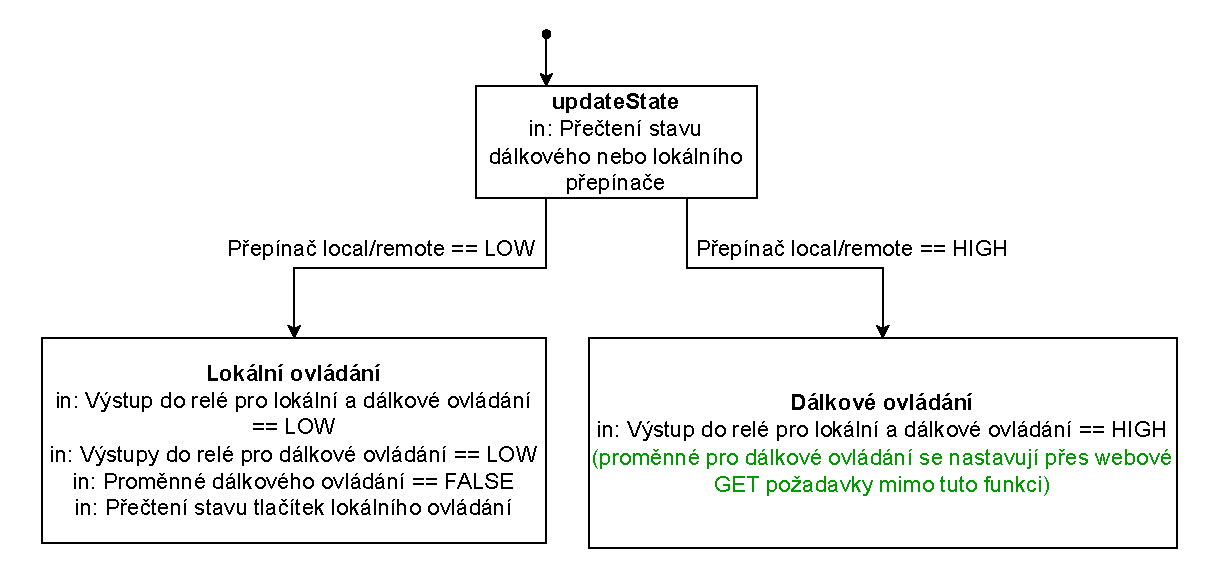
\includegraphics[width=1\linewidth]{images/StateFlow_Firmwaru_top.drawio.pdf}
    \caption{Začátek stavového diagramu}
    \label{fig:StateFlow_Firmwaru_top}
\end{figure}

Zde je vstup do stavového diagramu. Na začátku se přečte hodnota vstupního pinu který sleduje přepínač nastavující lokální nebo dálkové ovládání, který je fyzicky umístěn na desce. Na základě hodnoty se pokračuje buď to stavu kdy je zařízení ovládané lokálně nebo dálkově.

\dots
\begin{figure}[H]
    \centering
    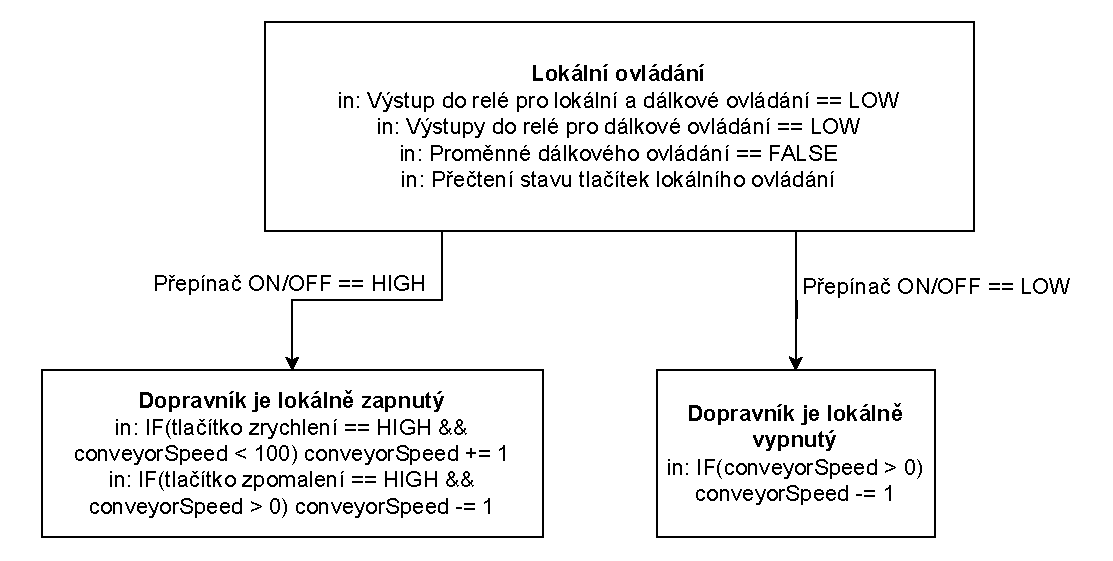
\includegraphics[width=1\linewidth]{images/StateFlow_Firmwaru_left.drawio.pdf}
    \caption{Strana stavového diagramu s lokálního ovládáním}
    \label{fig:StateFlow_Firmwaru_left}
\end{figure}

Ve stavu Local\_Controlled se nejdřív nastaví výstupní pin PIN\_OUT\_LOCALREMOTE. Nastavení výstupního pinu lokálního nebo dálkového ovládání vývojové desky na nízkou hodnotu zajistí, že ty tři přepínací (Form-C) relé na dolní straně blokového elektrického diagramu \ref{fig:SchemaDesky} budou připojené k lokální větvi ovládání. Dále se v tomto stavu nastaví všechny proměnné související s dálkovým ovládáním na false hodnotu. Nakonec se přečte stav vstupních pinů do vývojové desky související se stavem vypnuto/zapnuto, zrychlováním a zpomalováním a tyto stavy se uloží do proměnných, na základě kterých se bude rozhodovat co se dále stane ve stavovém diagramu.

\comment{Má cenu to takhle popisovat nebo je to zbytečné? }

\purpose{Pokud je tohle dobře popsané a má to cenu takhle popisovat tak zde i dál vysvětlím co se dál nachází ve zbylých částech stavového diagramu.}

\begin{figure}[H]
    \centering
    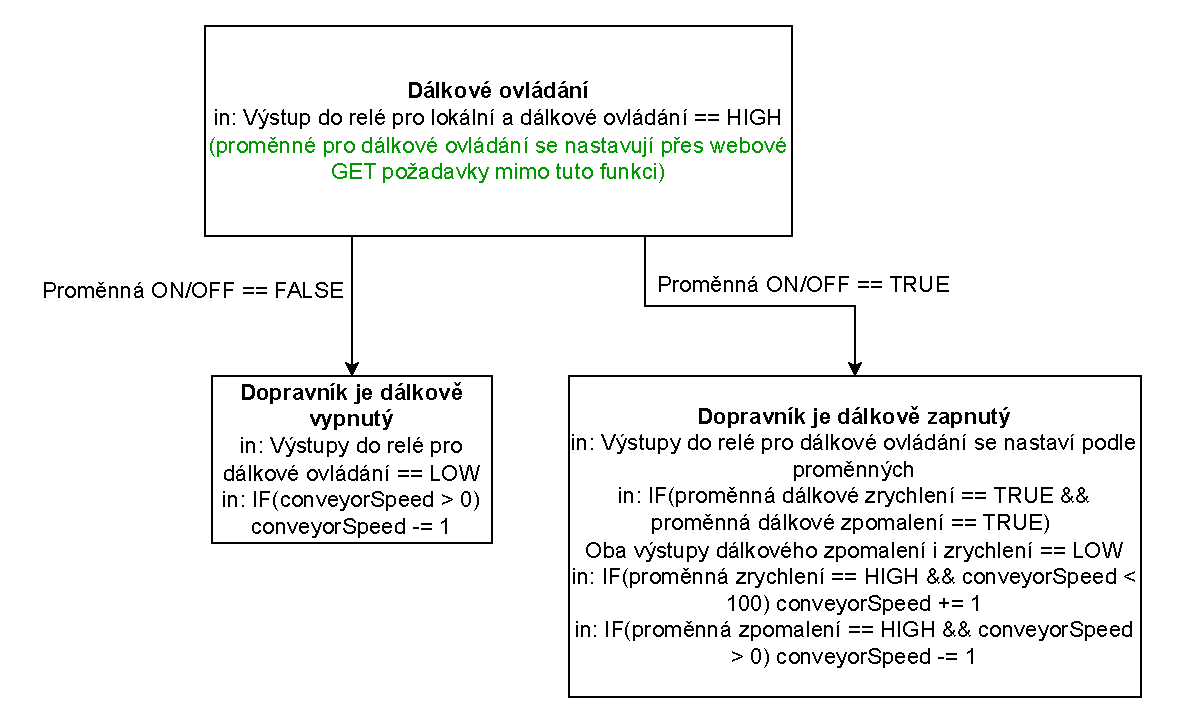
\includegraphics[width=1\linewidth]{images/StateFlow_Firmwaru_right.drawio.pdf}
    \caption{Strana stavového diagramu s dálkovým ovládáním}
    \label{fig:StateFlow_Firmwaru_right}
\end{figure}
\dots

\subsubsection{Jak aplikace aproximuje rychlost dopravníku}\label{sec:AproximaceRychlostiDopravniku}
\purpose{Vysvětlit jak se pomocí Tickeru aproximuje rychlost dopravníku}

Aplikace aproximuje rychlost dopravníku tak, že předpokládá že dopravník ovládaný frekvenčním měničem zrychluje lineárně - což je běžná praxe pro frekvenční měniče kvůli důvodům popsané v kapitole \ref{sec:JakFungujiFrekvencniMenice} a je to něco co jsem si potvrdil když jsem na dopravníku zkoušel funkčnost zařízení. Dává to smysl, protože tohle zrychlování je čistě softwarová záležitost frekvenčního měniče a tak není důvod proč by nebylo lineární. Během testování jsem zjistil, že frekvenční měnič má ramp up time sice nastavený na 10 sekund, ale za těch 10 sekund dosáhne $500 ot/min$. Pokud bych chtěl tedy zrychlit dopravník z nulové rychlosti na maximální rychlost 1500 otáček za minutu, musím počkat čas 3x větší než je jeden ramp up time. Dopravník stejnou rychlostí i zabrzďuje.

Samotná aproximace rychlosti je implementována ve funkci updateState, která je blíže vysvětlená ve kapitole \ref{sec:UpdateStateStavovyDiagram}. Aproximace je provedena hned po nastavení výstupních pinů v rámci updateState vývojové desky tím, že se přičte nebo odečte hodnota proměnné conveyorSpeed. Proměnná conveyorSpeed je nastavená jako celé číslo a reprezentuje procento rychlosti z maximální rychlosti. Jelikož se funkce updateState volá každých 0.3 sekundy a během každého zavolání se buďto zvýší conveyorSpeed pokud se zrychluje, nebo sníží conveyorSpeed pokud se zpomaluje, dosáhne maximální hodnoty 100 za 30 sekund, což je čas potřebný pro dosáhnutí maximální rychlosti dopravníku.

Funkce updateState se volá zaokrouhleně 3x za sekundu a takové rozlišení by mělo stačit pro to aby aproximace nenabývala hodnot drasticky mimo z důvodu např. rozpojení tlačítka těsně předtím než se provede updateState.

Tahle funkcionalita dává inženýrům co kontrolují dopravníky důležité informace o rychlosti i bez toho aby k dopravníku museli mít připojené zařízení jako BOP-2 z kapitoly \ref{sec:NastaveniOvladacihoPanelu} vysvětlující nastavení ovládacího panelu dopravníku.

\section{Software v mobilní aplikaci ($\Sigma$ = 5 stran)}\label{sec:SoftwareVMobilniAplikaci}
\purpose{V téhle sekci popíšu jak přesně funguje mobilní aplikace kterou jsem vytvořil a poznatky s tím spojené.}

Jak už jsem nastínil v \ref{sec:PopisFunkceSystemu} tak hlavní motivace proč navrhuji mobilní aplikaci je kvůli tomu aby nebylo potřeba mít extra zařízení pro ovládání dopravníků. Díky mobilní aplikaci můžu vytvořit zařízení které umožní dopravníky ovládat na vzdálenost 10-100 metrů (vzdálenost WiFi protokolu - \source{zdroj needed}) a stačí mi navrhnovat jenom zařízení které se připojí na dopravník a už nemusím navrhovat zařízení, které signály vysílá. To zmenšuje počet krabiček co musí zaměstnanci software tahat s sebou.

Výhodou mobilní aplikace je taková, že můžu na jedno místo dát všechny návody - můžu tak mít setup i všechno ovládání v rámci jedné aplikace což je rozhodně lepší než to mít v pdf dokumentu někde mimo. Pomáhá mi to tak na jeden z požadavků kdy jsem chtěl aby byl systém jednoduchý a intuitivní na používání.

\subsection{Architektura aplikace}
\purpose{Vysvětlit jakým způsobem jsem navrhoval architekturu aplikace a proč. Architektura = statická frontendová webová aplikace převedená do mobilní podoby pomocí WebView. Výhody jsou jednoduchost implementace GET requestů ve webové aplikaci. Zde taky přestavit React a Capacitor.}

Ta aplikace samotná je čistě frontendová (statická) webová aplikace postavná na Vite verzi Reactu. Capacitor tuhle aplikaci převádí do mobilní aplikace a kvůli tomu potřebuju používat některý balíčky spojený s capacitorem aby mi to umožnilo posílat webové požadavky na IP adresy nodeMCU serverů.

\textbf{Webová aplikace má tři URL adresy:}
\begin{itemize}
    \item Vstupní stránka - Tato stránka obsahuje hlavní část aplikace která umožňuje ovládání dopravníků.
    \item Setup - Tato stránka obsahuje návod jak dopravník nastavit aby s tímto zařízením správně fungoval.
    \item Help - Tato stránka obsahuje časté chyby které můžou nastat při používání zařízení a při nastavování dopravníků a snaží se poskytnout rady aby pomohla s vyřešením problémů.
\end{itemize}
Tyto URL adresy jsou převedené i do adres dostupných na mobilní aplikaci. Navigaci na tyto adresy zajišťuje header s navbarem jelikož v android WebView nelze zadávat URL adresy a tak musí navigace probíhat přes tlačítka na webu.

\purpose{Co je to React a proč se hodí na návrh této webové aplikace. Co je to HTML, CSS a JS. Co je to reaktivnost komponentů. Jak se react využívá. Možná sem přidat co je to tailwind a Lucide for React.}

React je web developmentovej framework a hodí se na návrh, protože přes node package manager už existují frameworky, který mi umožní webový aplikace portovat do mobilní aplikace - tenhle framework se jmenuje capacitor. Capacitor používá WebView (pro Android) nebo WKWebView (pro iOS) a díky tomu umožňuje zobrazit si webové aplikace na zařízení.\cite{CapacitorDocumentationFAQ}

Webovou aplikaci navrhuji, protože to, co chci aby dělala je aby jenom posílala GET požadavků na IP adresu mikrokontrolleru kterou hostuje NodeMCU, což je hodně jednoduchá věc na implementaci ve webové aplikaci.

\source{React může mít zase jako zdroj nějakou odbornou literaturu zaměřenou na react (pokud něco takového najdu) anebo online dokumentaci.}

\subsection{Použité knihovny a technologie v aplikaci (0.5 strany)}
\purpose{Vysvětlit co za frameworky (knihovny) jsem při developování aplikace použil aby to fungovalo co nejlépe}

\subsubsection{HTML, CSS a JS}

\subsubsection{TypeScript}

\subsubsection{Tailwind}

\subsubsection{DaisyUI}

\subsubsection{Lucide for React}

V rámci programování jsem používal několik rozšíření, které web developerům pomáhají v designu aplikací. Tím je \textbf{Tailwind}, což je rozšíření které umožňuje stylizovat kód webové aplikace pomocí vlastnosti className, kterou mají veškeré HTML prvky a tím není potřeba mít samostatné soubory v CSS (jazyk který webům dává jejich design). Na Tailwind navazuje rozšíření \textbf{DaisyUI}, které zjednodušuje celkový design aplikace tím, že mi umožňuje si nadefinovat barvy motivu aplikace v různých proměnných, díky čemuž je možné motiv měnit skrz změnu jedné promenné nastaveného motivu. Také umožňuje mít vlastní styl aplikace pokud má mobilní zařízení temný režim nebo světlý režim. S designem aplikace ještě pomáhalo rozšíření \textbf{Lucide pro React}, které obsahuje velké množství ikon pro různé prvky uživatelského rozhraní, jako je třeba ve tlačítkách ON/OFF, Add Conveyor, zrychlení, atd.

Aplikace ještě používá TypeScript, což je nadstavba JavaScriptu, která umožňuje definovat typy proměnných, což zvyšuje bezpečnost programu a zlepšuje zážitek z programování, vzhledem k tomu, že programátory upozorňuje na chyby v kódu, na které by JavaScript běžně neupozornil.

\subsection{Princip komunikace s NodeMCU servery}
\purpose{Co je to GET požadavek a jak se dá implementovat v JavaScriptu.}

\purpose{Jak se GET požadavek mění když používám capacitor}

\subsubsection{Co je to GET požadavek }
\purpose{Vysvětlit obecně jak fungují GET požadavky z web developmentu}

Aplikace bude ovládat nodeMCU servery přes posílání webových GET požadavků. GET požadavek je typicky například když do prohlížeče na PC zadám do URL adresy jakýkoliv název webu - tak to provádím GET požadavek na server, který je na IP adrese hostován. V tomhle případě jsou servery moje nodeMCU servery a místo PC zadávám požadavky přes webovou aplikaci.

V rámci nodeMCU se nastavují adresy na kterých server nějakým způsobem odpovídá. Během tohoto nastavení můžu nejenom určit jaká stránka se ukáže po zadání požadavku na získání informací z webové adresy, ale můžu tím spouštět i jakýkoliv jiný kód.

Typický test této funkce je pomocí GET požadavku na IP adresu rozsvítit LED diodu, která přes breadboard zapojená do výstupního pinu vývojové desky WEMOS D1 mini pro. Pokud je deska připojená ke stejné WiFi síti jako můj počítač, můžu na počítači zadat například adresu 192.168.0.144/ledON. NodeMCU server na tuto adresu odpoví tím, že změní stav LED diody v desce a až poté pošle zpátky HTML kód, který se mi zobrazí v prohlížeči. Takto je možné provádět jakýkoliv kód, který je nastaven aby se prováděl v rámci GET požadavků na jakoukoliv adresu.

V reactu se běžně GET požadavky provádí pomocí asynchronní funkce fetch. Asynchronní funkce jsou speciální funkce, během kterých můžeme používat speciální slovo "await". Tohle slovo způsobí, že Javascript počká než se daný příkaz dokončí a až poté bude pokračovat v provádění funkce. Tohle zamezuje vznik chyb v kódu, které můžou vznikat pokud se snažím dělat operace s proměnnými, které jsou zatím prázdné (jelikož ty data ještě například neposlal server).

V běžné react aplikaci by bylo možné posílat GET požadavky na nodeMCU server tímto způsobem:

\begin{lstlisting}[language=JavaScript, caption={Základní způsob posílání GET požadavků v JavaScriptu}, label={lst:JavaScriptFetchFunkce}]
async function getData() {
  const url = "https://example.org/products.json";
  try {
    const response = await fetch(url);
    if (!response.ok) {
      throw new Error(`Response status: ${response.status}`);
    }

    const json = await response.json();
    console.log(json);
  } catch (error) {
    console.error(error.message);
  }
}
\end{lstlisting}

\source{MDN web docs}

\subsubsection{Implementování GET requestů do aplikace}
\purpose{Vysvětlit proč normální GET requesty nefungují (Omezení z WebView) a jak je tedy implementovat. Taky zmínit že jsou implementované ve funkci sendCommand.}

GET požadavky není kvůli capacitoru možné posílat běžným způsbem, protože v android aplikaci nefunguje fetch funkce tak, jak se od ní očekává. Je ale možné použít balíček vytvořený komunitou capacitoru který se jmenuje CapacitorHttp (což bylo nedávno přidané do základního capacitor balíčku). je to balíček, který zjednodušuje posílání GET požadavků na servery v rámci Capacitor aplikací tím, že má metodu GET, která funguje jako běžný fetch požadavek typu GET, ale je upravený aby fungoval ve WebView mobilním prostředí.

Tímto způsobem se v aplikaci posílají GET požadavky:
\begin{lstlisting}[language=JavaScript, caption={Funkce sendCommand dostupná uvnitř vstupní stránky aplikace}, label={lst:SendCommandFunkce}]
    // pred zacatkem komponentu:
    import { CapacitorHttp } from "@capacitor/core";
    import { HttpOptions } from "@capacitor/core/types/core-plugins";

    // uvnitr komponentu se strankou aplikace:

      // Send a command to a specific conveyor and update its status
  const sendCommand = async (ip: string, command: string) => {
    try {
      const options: HttpOptions = {
        url: `http://${ip}/${command}`,
      };

      const response: any = await fetchWithTimeout(
        CapacitorHttp.get(options),
        3000 // Fail fast if conveyor is unresponsive
      );

      setErrorMessage(null);
      console.log(response);
      try {
        const responseData = await response.json();
        console.log("Response data:", responseData);
      } catch (error: any) {}
    } catch (error: any) {
      console.error("Command failed:", error);
      setErrorMessage(`Command failed for ${ip}: ${error.message}`);

      // Immediately mark the conveyor as offline when a command fails
      setConveyors((prevConveyors) =>
        prevConveyors.map((conv) =>
          conv.ip === ip ? { ...conv, isOnline: false } : conv
        )
      );
    }
\end{lstlisting}
Nejdřív je nutné si importovat HttpOptions a CapacitorHttp z capacitoru. Následně pokračuje definice komponentu, který obsahuje celou vstupní stránku aplikace. Uvnitř stránky aplikace je definovná funkce sendCommand.

Funkce sendCommand má jako vstupy IP adresu a adresu na kterou bude posílat GET požadavek. Princip je takový, že se do HttpOptions nastaví jako URL celá IP adresa i s adresou požadavku a to se pomocí CapacitorHttp.get funkce pokusí získat. Pokud byl požadavek úspěšně doručen, aplikace se bude pokoušet přeložit odpověď přes json syntaxi, ale to se často pokazí, protože aplikace v rámci některých odpověďí odpovídá i HTML kódem aby bylo možné ji ovládat i přes webový prohlížeč. Pokud se tedy přeložit odpověď nepovede, není to žádný problém a proto je v pořádku mít řádek s přeložením ze json souboru ve try catch bloku, který jakýkoliv error potlačí.

Pokud funkce nezíská odpověď do 3 sekund, kód aplikace pomocí fetchWithTimeout (moje vlastní funkce definovaná jinde v kódu) vyšle error, který do konsole vypíše, že požadavek z nějakého důvodu nebyl doručen a zároveň zobrazí i error v uživatelském rozhraní aplikace. Tohle je obzvlášť důležitá funkce, protože se uživateli v aplikaci ukáže error pokud v rámci času 3 sekund nodeMCU server neodpoví na požadavek - informuje to tedy o tom, že uživatel buďto zadal špatnou adresu, anebo odešel z dosahu ve kterém je nodeMCU server schopný se připojit na WiFi hotspot jeho mobilního zařízení. Tato implementace také vypíná možnost mačkat tlačítka, které ovládají dopravník, vzhledem k tomu, že by tlačítko vůbec nic nedělaly.

\subsection{Funkčnost aplikace (hodně stran)}
\purpose{Tady už vůbec neřešit jak ta aplikace vypadá, ale zaměřit se na to co ta aplikace dokáže a jak to dělá. Struktura hlavní stránky, správa seznamu dopravníků, ovládání dopravníků je zahrnuto v sendCommand, získávání a zobrazování stavu skrz sendCommand a stránky Setup a Help. TOHLE BUDE HLAVNÍ MEAT TÉHLE KAPITOLY}

Základ hlavní stránky je využívání reaktivnosti Reactu. Jelikož je aplikace dělaná v Reactu, je možné plynule přidávat dopravníky do seznamu bez toho aby se aplikace musela načítat pořád znovu. React nám také dává možnost ukládat IP adresy dopravníků do lokální paměti stránky a tak si aplikace vždy při spuštění načte data o dopravnících, které v aplikaci byly při posledním ukončení. React také umožňuje veškeré další funkce jako implementace GET požadavků a na základě těchto GET požadavků upravovat vzhled aplikace - jako například, že pokud GET požadavek nedostane úspěšnou odpověď do tří sekund, aplikace vyhodnotí daný nodeMCU server jako nefunkční a na základě toho uživatele vizuálně upozorní a vypne možnost se pokoušet o spojení s zařízením.

\subsubsection{Co funkci sendCommand používá}
\purpose{Vysvětlit proč je funkce sendCommand tak důležitá}

Funkci sendCommand používají všechny tlačítka aplikace, které je možné vidět na obrázku \ref{fig:MobilniAppScreenshots} (tlačítka ON/OFF, zrychlení a zpomalení dopravníku).

Funkce sendCommand se ale navíc sama provádí každé 2 sekundy pro každý dopravník přidaný do vstupní stránky aplikace. Provádí se tam GET požadavek na adresu /getData na adrese každého nodeMCU serveru. Tato adresa odpovídá s aktuální (aproximovanou) rychlostí dopravníku a s aktuálním stavem jestli je dopravník ovládaný lokálně nebo dálkově. Tato adresa už odpovídá pouze json souborem a díky tomu je důležité se i v rámci sendCommand pokoušet o přeložení odpovědi do javascript objektu pomocí příkazu $response.json()$. V případě těchto požadavků už program neselže s chybou a díky tomu uživatelské rozhraní aplikace získává informaci o rychlosti a stavu dopravníků, kterou může zobrazovat ve vstupní stránce jak je vidět na obrázku \ref{fig:MobilniAppScreenshots}.

\subsection{Design aplikace (1 strana)}
\purpose{Zde vysvětlit jak jsem postupoval při designování aplikace. Vysvětlit co je to header aplikace a že mám nějakej styling kterej je pro každý React komponenty aplikovanej automaticky.}

I přesto, že je aplikace programovaná jako webová aplikace jsem aplikaci designoval tak, aby vypadala v pořádku na mobilním zařízení. Vždy, když jsem aplikaci upravoval z grafické stránky, díval jsem se na ni přes \textit{Chrome developer tools}, ve kterých lze nastavit aby se web zobrazoval jako na mobilním zařízení. Tohle usnadnilo programování uživatelského rozhraní.

Aplikace má motiv pro světlé rozhraní telefonu (light mode) i pro temné rozhraní (dark mode). Zde je zobrazeno světlé rozhraní.

\begin{figure}[H]
    \centering
    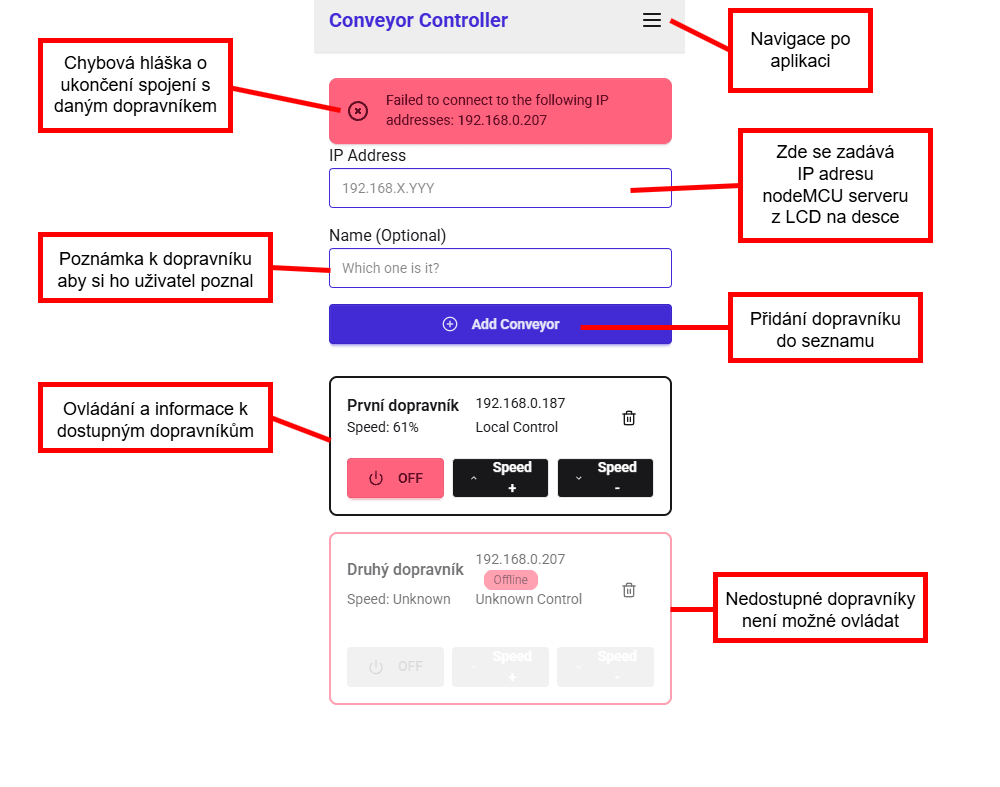
\includegraphics[width=0.9\linewidth]{images/LandingPage_Annot.png}
    \caption{Popis designu hlavní stránky aplikace}
    \label{fig:LandingPageAnnotated}
\end{figure}

\subsection{Konvertování webové aplikace do mobilní aplikace (0.5 strany)}\label{sec:KonvertovaniWeboveAplikaceDoMobilni}

\purpose{Zmínit že je možné react aplikaci pomocí Android Studia portnout do .apk souboru který používá WebView a dále co je to CORS a že operační systém androidu defaultně zakazuje HTTP requesty.}

V téhle části asi jenom zmíním, že je možné tuhle react aplikaci přes android studio portnout do .apk souboru, který se dá nainstalovat na android telefonech. Přes android studio je i možné aplikaci certifikovat a uploadnout na play store, ale to nemám zapotřebí, protože nechci aby tuhle aplikaci měli lidi co nejsou z Honeywellu.

Tady taky můžu zmínit co je to CORS (Cross Origin Resource Sharing), což je protokol který zamezuje serverům jako je nodeMCU v komunikaci s ostatními klienty kvůli bezpečnosti. Vzhledem k tomu, že IP adresu nodeMCU serverů může být úplně jakákoliv, musím CORS nastavit na možnost odpovídat na jakékoliv GET requesty z jakékoliv adresy, což teoreticky není doporučované kvůli snížení bezpečnosti proti útokům. V praxi to je ale úplně jedno, protože ten nodeMCU server je jenom na mém hotspotu a odjinud z internetu není dostupný.

Druhá věc co můžu zmínit je, že operační systém android zařízení defaultně zakazuje všechny HTTP requesty a umožňuje jenom HTTPS requesty. HTTPS ale také nemá cenu zavádět na nodeMCU serveru protože je na lokální síti. V rámci aplikace musím ale HTTP requesty povolit tím, že to napíšu do AndroidManifest.xml filu.

\source{Tady budou zdroje asi jenom online - capacitor dokumentace, android studio dokumentace, CORS dokumentace}

\subsubsection{Požadavky na React aplikaci aby se dala konvertovat}\label{sec:PozadavkyNaReactAplikaceAbySeDalaKonvertovat}
\purpose{Vysvětlit co je potřeba splnit aby se aplikace dala konvertovat do .apk}

Abych tu react aplikaci mohl konvertovat pomocí kapacitoru, musí to být statická webová aplikace - tedy jen aplikace s frontendem bez serverových endpointů. Na každou routu musí existovat nějaký odkaz v navigaci aplikace (protože v capacitor aplikaci nemůžu jen tak zadat URL). A možná další věci.

Kvůli těm URL adresám musí v aplikaci i být header s navbarem. Header obecný název pro tu část aplikace co je hned nahoře a většinou obsahuje navigační prvky - jako navbar, což je část aplikace která obsahuje tlačítka přes které se lze dostat na další stránky.

Ještě zmínit jakým způsobem mají být řešení odkazy v single page aplikaci aby bylo možný se skrz ni navigovat plynule - tedy že nepoužívat anchor tagy.

\source{Asi capacitor docs.}

\subsubsection{Postup konvertování webové aplikace}
\purpose{Už nepsat teorii jak by se dala aplikace zkonvertovat jako ve kapitole \ref{sec:KonvertovaniWeboveAplikaceDoMobilni} ale specificky napsat jak jsem postupoval při konvertování aplikace krok za krokem.}

Pro konvertování jsem použil android studio verze x.x. atd.

Konvertování webové aplikace do mobilní aplikace je postup o několika krocích který využívá kapacitor inicializovaný v projektu a následně Android Studio, které je potřeba pro překonvertování projektu z kapacitoru do souboru instalovaného na android zařízeních o příponě .apk.

\begin{itemize}
    \item Začíná se v nejnovější verzi React webové aplikace.
    \item Tuto aplikaci člověk musí nejdříve postavit do produkční verze pomocí příkazu \textit{npm run build}.
    \item Dále je potřeba aplikaci zesynchronizovat s kapacitorem pomocí příkazu \textit{npx cap sync}.
    \item Nyní je potřeba si otevřít nainstalovaný program android studio, co je možné udělat rovnou z konsole pomocí příkazu \textit{npx cap open android}.
    \item Nakonec je v android studio potřeba znovu postavit aplikaci do produkční verze pomocí příkazu build.
\end{itemize}

Na konci tohoto procesu je dostupný soubor přípony \textit{.apk}, který je možné si poslat na android mobilní zařízení a tam nainstalovat.

Aplikace nevyžaduje žádné další nastavování.

\section{Vytvoření schránky pro desku (1 strana)}
\purpose{V téhle sekci bude popis jak jsem postupoval při návrhu schránky pro desku, která obsahuje i tlačítka.}

Myšlenka při návrhu schránek pro desku byla taková abych ji mohl vytisknout v běžných podmínkách pomocí 3D tiskárny Bambu Lab A1 Mini, kterou mám doma. Hlavní důvod proč jsem zvolil 3D tisk jako technologii bylo, že těchto schránek bude ve finále vytisknutých asi 5 kusů a tak není potřeba zajišťovat sériovou výrobu. Navíc je to pro schránky na desky plošných spojů levné řešení, které dosahuje dostatečné kvality provedení. Nároky na schránku jsou základní - je důležité mít možnost ji rozdělat aby byla možná údržba desky, ale jinak nemá zvláštní nároky, vzhledem k tomu, že bude vytažená pár týdnů do roku.

Modelovací software pro návrh schránky pro desku jsem zvolil online CAD Onshape. Do toho jsem si nahrál 3D model desky plošných spojů v .STL formátu který mi vygeneroval KiCAD pomocí 3D prohlížeče a na základě tohoto modelu jsem začal modelovat schránku na míru pro moji desku. Rozhodl jsem se, že schránka bude vytvořena ze dvou hlavních částí a že bude bez šroubů, aby bylo možné na ni jednodušeji prototypovat zařízení, ale zároveň bylo cílem aby stále držela dohromady během používání, pokud zrovna není potřeba ji otevírat.

To se mi povedlo pomocí dvou částí. Do dolní části je možné zajet desku plošných spojů a díky tomu deska ve schránce dobře drží. V dolní části je také otvor na kabely které jsou uchycené v desce plošných spojů. poté je možné vzít celou dolní část a zajet ji do horní části schránky, která obsahuje prostor pro tlačítka, LCD display a díru na našroubování antény pro zlepšení připojení k WiFI. Nakonec schránka obsahuje ještě jednu část a to je brána, který dolní část desky zajistí aby nevyjížděla z horní části.

\begin{figure}[H]
    \centering
    \begin{subfigure}[t]{0.48\textwidth}
        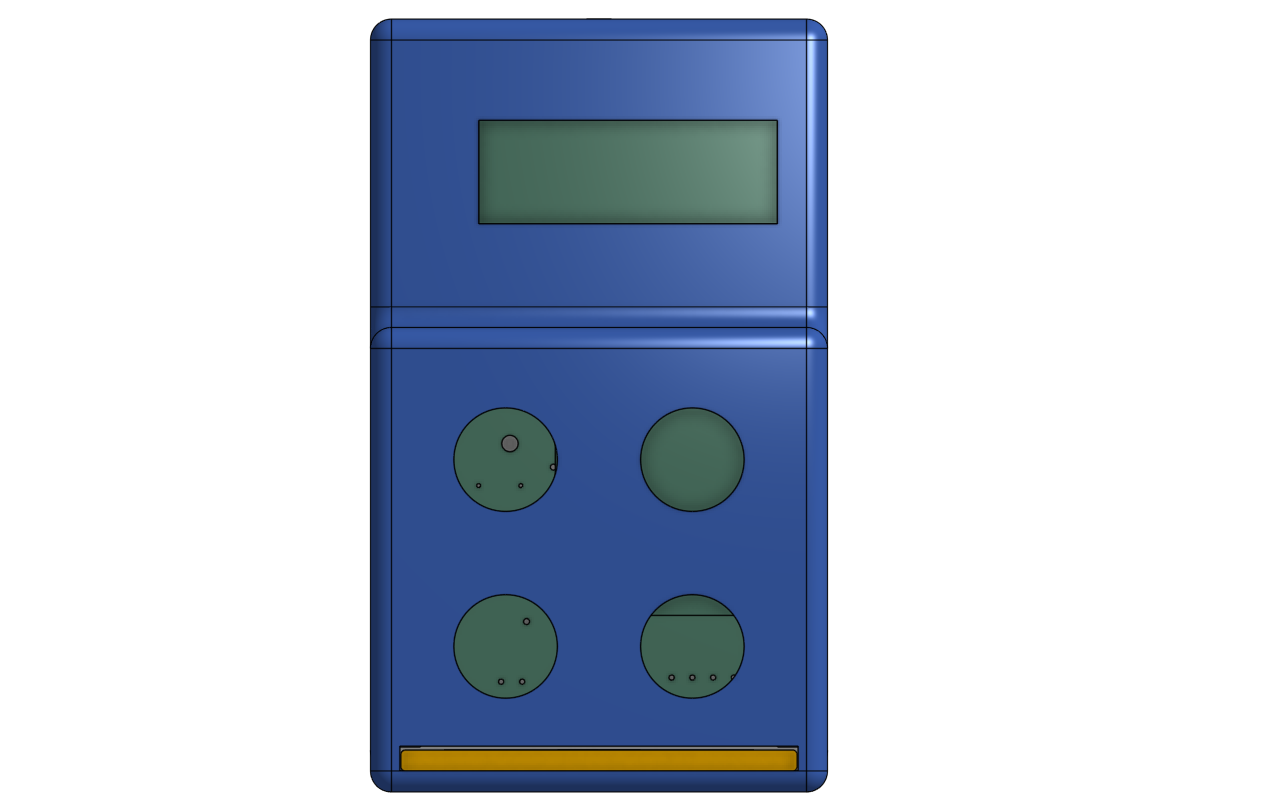
\includegraphics[width=\textwidth]{images/krabickaTop.png}
        \caption{Pohled shora na schránku}
        \label{fig:krabickaTop}
    \end{subfigure}%
    \hfill
    \begin{subfigure}[t]{0.48\textwidth}
        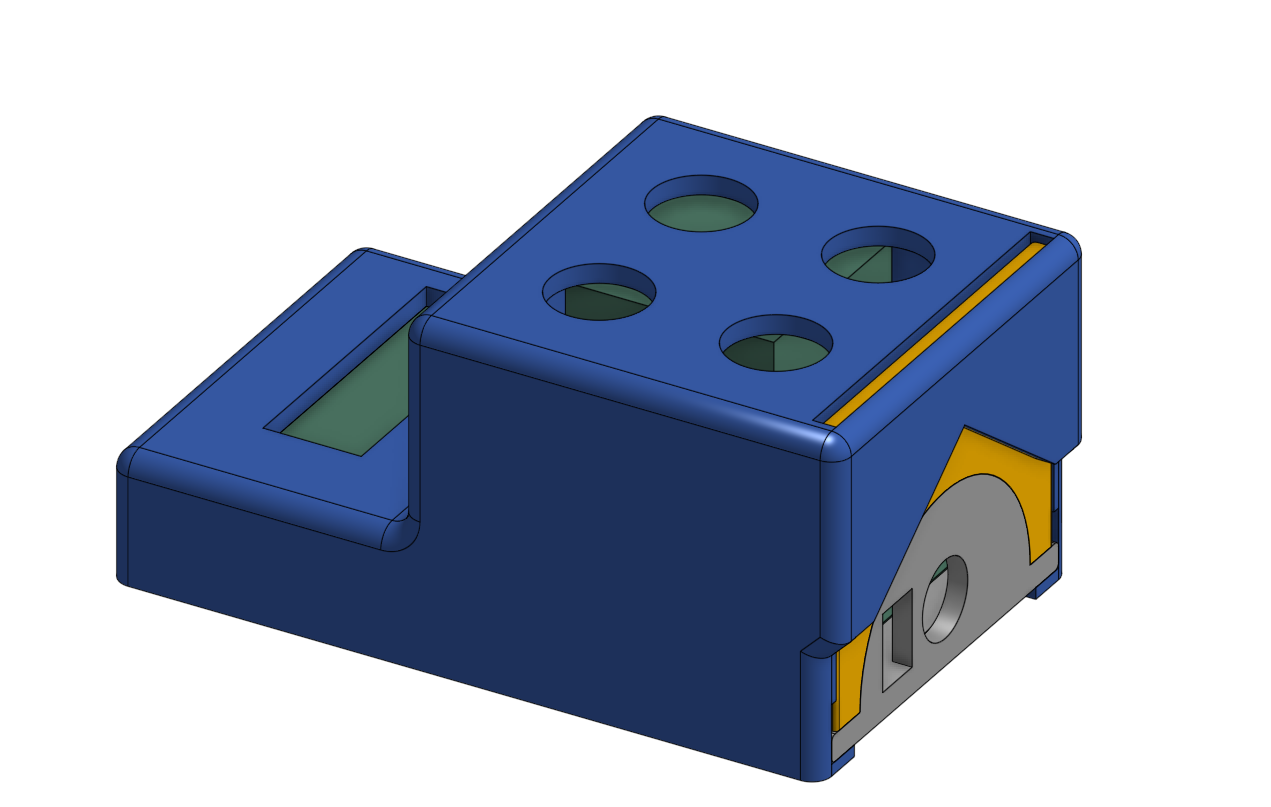
\includegraphics[width=\textwidth]{images/KrabickaZBoku.png}
        \caption{Pohled z boku na schránku}
        \label{fig:KrabickaZBoku}
    \end{subfigure}
    \caption{Model schránky pro desku plošných spojů}
    \label{fig:krabickaObaPohledy}
\end{figure}

Po vytvoření modelů v Onshape jsem si pomocí Bambu Studio do tiskárny poslal desku a vytiskl jsem ji z bílého PETG materiálu značky SUNLU, který jsem vybral díky jeho vyšší robustnosti než PLA, ale zároveň nepotřebuje složitější procesy a hardware pro tisknutí. Během tisknutí jsem filament sušil kvůli notoricky známým problémům PETG a vlhkosti filamentu.

\section{Kompletace řešení (2 strany)}
\purpose{Tady bude postup kompletace celého zařízení a k tomu obrázky, které blíže popisují kde jsou jednotlivé části.}

Při kompletaci jsem připájel všechny součástky na desku a vložil jsem do desky dvě součástky, které jsou vyjímatelné - vývojovou desku WEMOS D1 Mini Pro a LCD Displej. Tyto součástky jsou vyjímatelné protože to jsou složité součástky sestavené z více různých částí, ale nejsou ve formě uzavřených integrovaných obvodů. Kvůli tomu existuje riziko, že by nebyly správně kompletované a v tom případě se hodí mít možnost je jednoduše oddělat a odstranit na nich problémy. Vývojová deska se navíc musí často oddělávat aby bylo možné na ni nahrávat kód při tvoření a LCD má zezdola trimmer, kterým se mění viditelnost textu.

\begin{figure}[H]
    \centering
    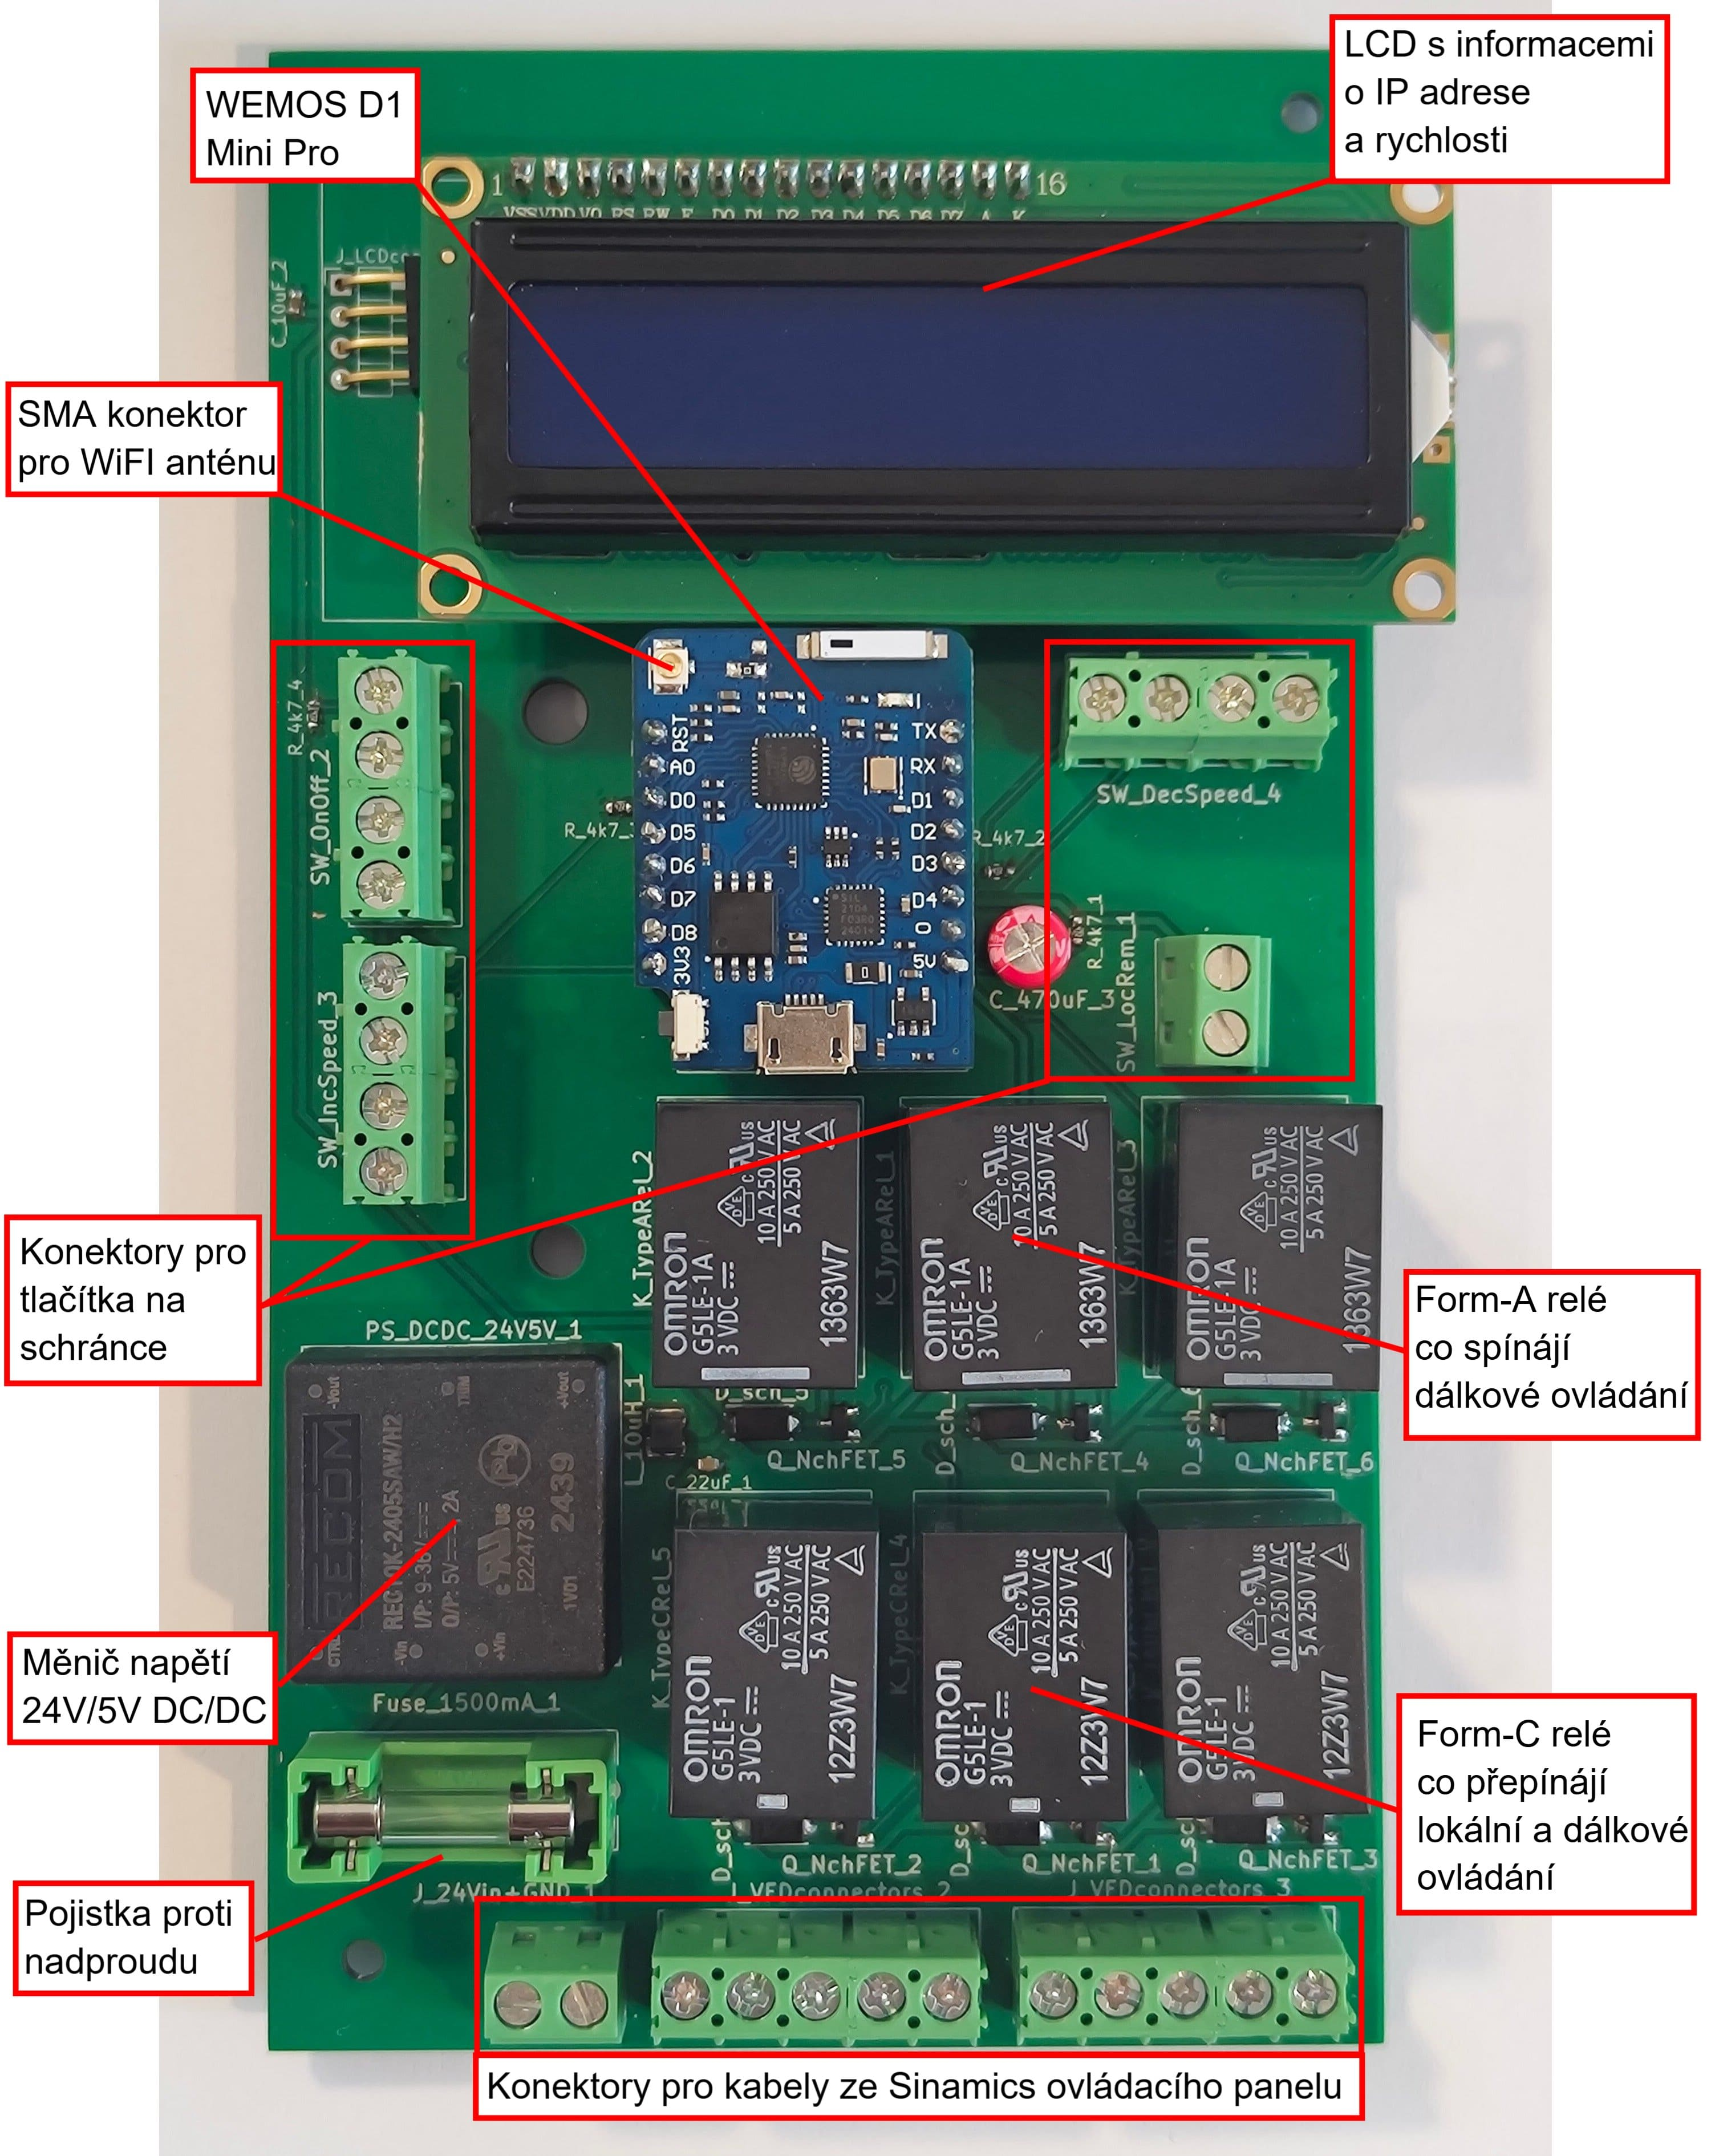
\includegraphics[width=0.95\linewidth]{images/PCB_Final_annotated.jpg}
    \caption{Finální podoba desky plošných spojů}
    \label{fig:PCBFinal}
\end{figure}

Následně stačí jen přidělat kabely do desky na šroubovací konektory a složit schránku na desku. V tomto stavu by mělo zařízení být připravené na připojení na dopravník jako to je v obrázku \ref{fig:PrincipFunkceZarizeni}. Desku je možné napájet buďto z ovládacího panelu frekvenčního měniče, což je doporučené, jelikož jsou do tohoto ovládacího panelu připojené i další kabely vycházející ze zařízení, ale je možné desku napájet i z jakéhokoliv zdroje napětí, který má napětí mezi $9-48V$ a je schopný dodávat proud do hodnot asi $0.5A$.



